\documentclass[11pt,a4paper]{article}

\usepackage[T1]{fontenc}
\usepackage[utf8]{inputenc}
\usepackage[english]{babel}
\usepackage{amsmath,amssymb,mathtools,geometry,booktabs,xcolor,tikz,hyperref,listings}

\usetikzlibrary{arrows.meta,positioning,shapes.geometric,calc}
\geometry{margin=22mm}
\definecolor{navy}{RGB}{18,49,88}
\hypersetup{colorlinks=true,linkcolor=navy}
\lstset{basicstyle=\ttfamily\small,breaklines=true,frame=single}
\title{Neural Networks and Numerical Solvers\\\large Concepts, Methods and Implementations}
\author{Frédéric Magoulès}
\date{November 2026}

\begin{document}\maketitle\tableofcontents\newpage

\section{Organization of resources and practical exercises}

The \texttt{reference/} directory contains the \textbf{executable solutions}: complete notebooks used to check implementations and reproduce numerical experiments.
The \texttt{student/} directory contains the participants' versions, with selected code sections to complete.
The \texttt{instructor/} directory contains \textbf{conceptual explanations}: mathematical foundations, numerical interpretation, diagrams, and teaching notes. It supplements rather than replaces the executable solutions.
\begin{center}\begin{tabular}{ll}\toprule Notebook & Topic \\\midrule
\texttt{model\_architecture} & MLP, CNN, kNN graph, EdgeConv and GNN\\
\texttt{training\_process} & weak and strong divergence constraints\\
\texttt{hybrid\_corrector} & residual-to-error learning\\
\texttt{hybrid\_accelerator} & right-hand-side-to-solution learning\\\bottomrule\end{tabular}\end{center}

\section{Supervised learning with PyTorch}

\subsection{Principles and implementation of training}

We are given $N$ input--target pairs $(x_i,y_i)$, where $x_i$ is an input and $y_i$ is the expected output. The goal is to learn a function that predicts $y_i$ from $x_i$. The neural network $F_\theta$ represents this function: $F$ denotes the model mapping, while $\theta$ is the collection of trainable parameters (weights and biases). The index $i$ identifies a sample, and $N$ is the number of training samples.

We seek optimal parameters $\theta^*$ by minimizing a loss function $\mathcal L$, for example the mean squared error:
\[
\boxed{\theta^*=\arg\min_\theta\mathcal L(\theta),\qquad
\mathcal L(\theta)=\frac{1}{N}\sum_{i=1}^N\|F_\theta(x_i)-y_i\|_2^2.}
\]
The norm $\|\cdot\|_2$ measures the discrepancy between prediction and target. An epoch is one full pass through the training dataset. The dataset is split into mini-batches; for each mini-batch, a forward pass computes predictions, the loss measures their errors, backpropagation computes gradients, and the optimizer updates the parameters. The learning rate controls the size of these updates.
\begin{lstlisting}[language=Python]
model = NeuralNetwork()  # A user-defined torch.nn.Module
optimizer = torch.optim.Adam(model.parameters(), lr=1e-3)
loss_fn = torch.nn.MSELoss()
loader = DataLoader(TensorDataset(X_train, Y_train),
                    batch_size=32, shuffle=True)
for epoch in range(150):
    model.train()
    for xb, yb in loader:
        pred = model(xb)        # Forward pass
        loss = loss_fn(pred,yb) # Objective function
        optimizer.zero_grad()  # Reset accumulated gradients
        loss.backward()        # Automatic differentiation
        optimizer.step()       # Update parameters
\end{lstlisting}
\paragraph{Key distinction.} \texttt{loss.backward()} computes gradients but does not update weights; \texttt{optimizer.step()} updates them. Plain gradient descent uses $\theta^{k+1}=\theta^k-\eta\nabla_\theta\mathcal L_B(\theta^k)$, while Adam uses adaptive moments. A validation curve, computed using data not used during training, makes it possible to assess the network's ability to make predictions at previously unseen points and to detect potential overfitting.

\subsection{Introductory example: approximating a sine function with an MLP (\textit{mlp\_sine\_intro})}

Consider the scalar function
\[y(x)=\sin(2\pi x),\qquad x\in[0,1].\]
The network $F_\theta:\mathbb R\to\mathbb R$ has two hidden layers of 32 neurons with \texttt{Tanh} activations. The mean squared error is minimized over pairs $(x_i,y_i)$:
\[\mathcal L(\theta)=\frac1N\sum_{i=1}^{N}|F_\theta(x_i)-\sin(2\pi x_i)|^2.\]
The program uses Adam, mini-batches of 32 samples and 200 epochs. It plots training and validation losses versus epochs, as well as the exact function and the MLP prediction. Validation data are distinct from training data.
\paragraph{Running the example.} From \texttt{instructor/}, run \texttt{python mlp\_sine\_intro.py} (dependencies: NumPy, PyTorch, Matplotlib), or execute \texttt{mlp\_sine\_intro.ipynb}. The figure \texttt{mlp\_sine\_results.png} is saved automatically.
\paragraph{Connection to later notebooks.} This example introduces the \texttt{forward} $\rightarrow$ \texttt{loss} $\rightarrow$ \texttt{backward} $\rightarrow$ \texttt{step} sequence. \texttt{model\_architecture} compares network architectures; \texttt{training\_process} introduces physical constraints; \texttt{hybrid\_corrector} and \texttt{hybrid\_accelerator} learn errors and solutions of linear systems, respectively.

\section{Neural network architectures: MLP, CNN and GNN (\textit{model\_architecture})}

In \texttt{model\_architecture}, the MLP operates on a flattened
or pointwise representation, the CNN exploits local convolutions
on an ordered grid, and the GNN aggregates messages using
\texttt{edge\_index}.
The graph is built from irregular coordinates by
\texttt{create\_knn\_graph}, with $k=5$ by default.
Each mesh edge is represented in both directions to allow
information to propagate in both directions.
For each node $i$, messages from its neighboring nodes are
computed and then aggregated as follows:
\[
m_{ij} = \operatorname{MLP}_{\theta}([h_i,h_j]),
\qquad
h'_i = \frac{1}{|\mathcal{N}(i)|}
\sum_{j \in \mathcal{N}(i)} m_{ij},
\]
where:
\begin{itemize}
    \item $i$ denotes the node whose features are to be updated;
    \item $j$ denotes a neighboring node of $i$;
    \item $h_i$ and $h_j$ are the feature vectors associated
    with nodes $i$ and $j$, respectively;
    \item $[h_i,h_j]$ denotes the concatenation of these
    two vectors;
    \item $\operatorname{MLP}_{\theta}$ is a multilayer
    perceptron whose trainable parameters are denoted by
    $\theta$;
    \item $m_{ij}$ is the message computed from the features
    of nodes $i$ and $j$, intended for node $i$;
    \item $\mathcal{N}(i)$ denotes the set of neighboring
    nodes of $i$, and $|\mathcal{N}(i)|$ is the number
    of these neighbors;
    \item $h'_i$ is the updated feature vector of node $i$,
    obtained by averaging the received messages.
\end{itemize}

Duplicate directed edges should be avoided, as they would
cause certain messages to be counted multiple times,
thereby changing their relative weights in the
mean aggregation.

This operation constitutes a message-passing step in
a graph neural network (GNN).
The GNN has three \texttt{EdgeConv} layers. Unless globally informative features are provided, three message-passing steps cannot transmit messages beyond three graph hops. Here, the distance to the source is already a node feature, so available information cannot be characterized solely by the number of layers.
\begin{center}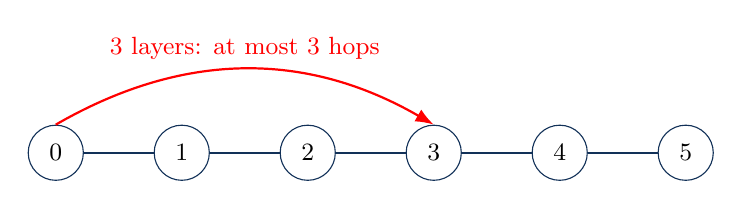
\begin{tikzpicture}[>=Latex, every node/.style={font=\small}]
\foreach \x/\lab in {0/0,1.6/1,3.2/2,4.8/3,6.4/4,8/5}{\node[circle,draw=navy,minimum size=7mm] (n\lab) at (\x,0) {\lab};}
\foreach \a/\b in {0/1,1/2,2/3,3/4,4/5}{\draw[thick,navy] (n\a)--(n\b);}
\draw[->,thick,red] (n0.north) to[bend left=30] node[above] {3 layers: at most 3 hops} (n3.north);
\end{tikzpicture}\end{center}

\section{Learning-based acceleration of numerical solvers}

\subsection{Discrete problem formulation}

Consider a Poisson problem with homogeneous Dirichlet boundary conditions:
\[-\Delta u=f\quad\text{in }\Omega,\qquad u=0\quad\text{on }\partial\Omega.\]
After eliminating boundary degrees of freedom, the discretization gives
\[Au=f,\qquad u^*=A^{-1}f.\]
The notation $A^{-1}$ is \emph{conceptual}: the notebooks obtain reference solutions with a sparse direct solver; they do not form an inverse matrix. The operator $A$ is fixed by the mesh, discretization, and boundary conditions. The neural networks approximate its action on a \emph{distribution} of input vectors.

\subsection{Jacobi method and smoothing properties}

Write $A=D-(L+U)$, where $D$ is the diagonal and $L+U=D-A$. Jacobi reads
\[u^{k+1}=u^k+D^{-1}(f-Au^k),\qquad e^{k+1}=(I-D^{-1}A)e^k.\]
The iteration matrix is $T_J=I-D^{-1}A$. For the model Laplacian on a regular grid, Jacobi damps certain oscillatory error components rapidly, whereas smooth components may decay slowly. This is not a universal claim for arbitrary matrices: damping depends on $A$ and its modes.

\subsection{Learning-based solution acceleration (\textit{hybrid\_accelerator})}

In \texttt{hybrid\_accelerator}, the training pairs are $(f,u^*)$ with $Au^*=f$. The CNN $G_\theta$ learns
\[\boxed{G_\theta(f)\simeq A^{-1}f=u^*.}\]
Its output is used \emph{once} as the initial guess $u^0=G_\theta(f)$; standard Jacobi iterations follow. This notebook does not use the CNN at each iteration.
\begin{center}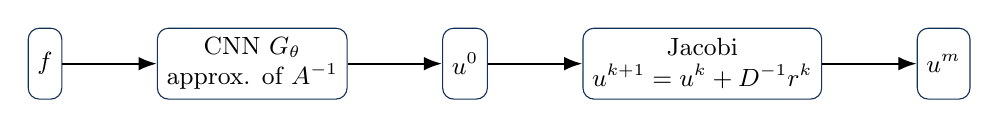
\begin{tikzpicture}[node distance=12mm,>=Latex, every node/.style={font=\small},box/.style={draw=navy,rounded corners,minimum height=9mm,align=center}]
\node[box] (f) {$f$};\node[box,right=of f] (cnn) {CNN $G_\theta$\\approx. of $A^{-1}$};\node[box,right=of cnn] (u) {$u^0$};\node[box,right=of u] (jac) {Jacobi\\$u^{k+1}=u^k+D^{-1}r^k$};\node[box,right=of jac] (res) {$u^m$};
\draw[->,thick] (f)--(cnn);\draw[->,thick] (cnn)--(u);\draw[->,thick] (u)--(jac);\draw[->,thick] (jac)--(res);
\end{tikzpicture}\end{center}

\subsection{Learning-based error correction (\textit{hybrid\_corrector})}

For an approximate solution $u^k$, define
\[r^k=f-Au^k,\qquad e^k=u^*-u^k.\]
The identity $Ae^k=r^k$ implies
\[\boxed{e^k=A^{-1}r^k,\qquad C_\theta(r^k)\simeq e^k.}\]
The \texttt{hybrid\_corrector} notebook learns $(r^k,e^k)$ pairs after a randomly chosen number of Jacobi iterations. After \texttt{cnn\_at\_step} iterations, it applies one additive correction:
\[u^{k,+}=u^k+C_\theta(r^k),\qquad e^{k,+}=e^k-C_\theta(r^k),\]
then resumes Jacobi. An exact correction would give $u^{k,+}=u^*$; a learned approximation generally leaves nonzero error and residual.
\begin{center}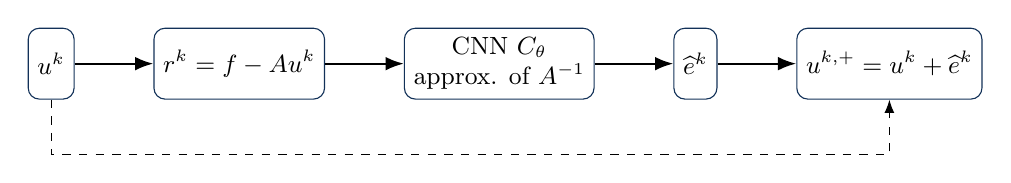
\begin{tikzpicture}[node distance=10mm,>=Latex, every node/.style={font=\small},box/.style={draw=navy,rounded corners,minimum height=9mm,align=center}]
\node[box] (uk) {$u^k$};\node[box,right=of uk] (r) {$r^k=f-Au^k$};\node[box,right=of r] (cnn) {CNN $C_\theta$\\approx. of $A^{-1}$};\node[box,right=of cnn] (e) {$\widehat e^k$};\node[box,right=of e] (plus) {$u^{k,+}=u^k+\widehat e^k$};
\draw[->,thick] (uk)--(r);\draw[->,thick] (r)--(cnn);\draw[->,thick] (cnn)--(e);\draw[->,thick] (e)--(plus);\draw[->,dashed] (uk.south) -- ++(0,-.7) -| (plus.south);
\end{tikzpicture}\end{center}

\subsection{Normalization of input and output data}

In \texttt{hybrid\_accelerator}, $s_f=\sqrt{\operatorname{mean}(f_{\rm int}^2)}+10^{-10}$ and the network is trained on $(f/s_f,u^*/s_f)$. In \texttt{hybrid\_corrector}, $s_r=\sqrt{\operatorname{mean}(r_{\rm int}^2)}+10^{-10}$ and the pairs are $(r/s_r,e/s_r)$. At inference, the prediction is multiplied by the same factor. This respects the homogeneity of the target linear operator without guaranteeing that the learned CNN itself is linear.

\section{Learning under physical constraints (\textit{training\_process})}

The source notebook is named \texttt{training\_process.ipynb}. It reconstructs a two-dimensional velocity field $v=(v_x,v_y)$.

\subsection{Weak enforcement of constraints: divergence penalization}

The network directly outputs $v_\theta(x,y)$, with loss
\[\boxed{\mathcal L_{\rm weak}=\frac1N\sum_{i=1}^N\|v_\theta(x_i)-v_i\|^2+\lambda_{\rm div}\frac1N\sum_{i=1}^N|\partial_x v_{\theta,x}(x_i)+\partial_y v_{\theta,y}(x_i)|^2.}\]
Automatic differentiation must be enabled for the coordinates. Divergence is penalized, not identically zero; the trade-off depends on $\lambda_{\rm div}$.

\subsection{Strong enforcement of constraints: stream-function formulation}

A second network learns a scalar potential $\psi_\theta(x,y)$ and constructs
\[\boxed{v_\theta=(\partial_y\psi_\theta,-\partial_x\psi_\theta).}\]
For sufficiently smooth $\psi_\theta$,
\[\nabla\cdot v_\theta=\partial_x\partial_y\psi_\theta-\partial_y\partial_x\psi_\theta=0.\]
This is a structural identity independent of penalty weights, although numerical discrepancies can remain. Automatic differentiation required to construct $v$ must remain active during inference.
\begin{center}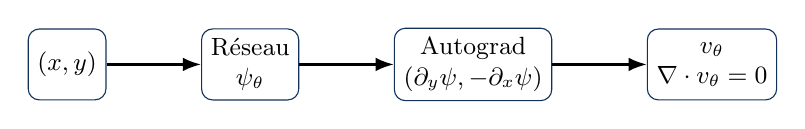
\begin{tikzpicture}[node distance=12mm,>=Latex,box/.style={draw=navy,rounded corners,align=center,minimum height=9mm},every node/.style={font=\small}]
\node[box] (xy) {$(x,y)$};\node[box,right=of xy] (nn) {Réseau\\$\psi_\theta$};\node[box,right=of nn] (grad) {Autograd\\$(\partial_y\psi,-\partial_x\psi)$};\node[box,right=of grad] (v) {$v_\theta$\\$\nabla\cdot v_\theta=0$};
\draw[->,thick] (xy)--(nn);\draw[->,thick] (nn)--(grad);\draw[->,thick] (grad)--(v);
\end{tikzpicture}\end{center}

\section{Annotated Solutions to the Practical Exercises}

The answers below follow the ten exercises in the notebooks in
\texttt{student/}. The corresponding implementations are available
in \texttt{reference/}. Exact numerical observations depend on
training and running the notebooks.

\subsection{Exercise 1 --- MLP forward pass}

\noindent \textbf{Question.} Reconstruct \texttt{forward}, compare the inductive
biases of an MLP and a CNN, and discuss generalization to a new
source location.
\\

\noindent \textbf{Annotated solution.} In \texttt{SpatialMLP}, the input
\texttt{x\_onehot} has shape $(B,N)$, where $B$ is the batch size
and $N$ is the number of grid points (64 by default). Each point
receives two features: its coordinate $x_i$ and the source
indicator at that point. Concatenation gives $(B,N,2)$, which
is reshaped to $(BN,2)$. The fully connected network applies
$2\to64\to64\to1$ and reshapes the output to $(B,N)$.
This MLP acts pointwise and does not directly mix neighboring
points during its forward pass. A CNN instead applies shared
local filters along the grid, introducing locality and
translation-related inductive biases (subject to boundary
effects). Good predictions at source locations seen in
training do not guarantee good predictions at unseen
locations; this must be checked on test examples.

\subsection{Exercise 2 --- kNN graph construction}

\noindent \textbf{Question.} Implement \texttt{create\_knn\_graph} with
symmetric directed connections and explain reachable neighborhoods.
\\

\noindent \textbf{Annotated solution.} For each node $i$, compute distances
to all other nodes, exclude $i$, and select its $k$ nearest
neighbors. For each selected neighbor $j$, insert both
$(i,j)$ and $(j,i)$ in \texttt{edge\_index}.
These two directions are not duplicates. However, if $i$
and $j$ select one another, an identical directed edge
may be inserted more than once. Under the \texttt{mean}
aggregation of \texttt{EdgeConv}, repeated occurrences
are counted multiple times and may change the average.
One message-passing layer can receive information from
immediate neighbors, two layers from nodes at graph
distance at most two, and so on, without guaranteeing
that all information is preserved.

\subsection{Exercise 3 --- EdgeConv message}

\noindent \textbf{Question.} Construct messages from source and target
node features and interpret GNN depth.
\\

\noindent \textbf{Annotated solution.} The method \texttt{message(x\_i,x\_j)}
concatenates the target feature vector $h_i$ and source
feature vector $h_j$:
\[
m_{ij}=\operatorname{MLP}_{\theta}([h_i,h_j]),\qquad
h_i'=\frac{1}{|\mathcal N(i)|}\sum_{j\in\mathcal N(i)}m_{ij}.
\]
Here $h_i,h_j$ are node feature vectors, $\theta$ denotes
MLP parameters, $m_{ij}$ is the message received by node $i$,
and $\mathcal N(i)$ denotes its neighbors (without repeated
entries in this mathematical expression). Three
message-passing layers provide structural dependence on
features at graph distance at most three. Local propagation
alone cannot access arbitrarily distant node features.
This limitation concerns graph propagation, not global
information already encoded in input features.

\subsection{Exercise 4 --- Residual-to-error dataset}

\noindent \textbf{Question.} Generate $(r,e)$ pairs, prove $Ae=r$,
and explain shared normalization.
\\

\noindent \textbf{Annotated solution.} For $Au^*=f$, an approximation $u$
after a random number of Jacobi steps (0 to 59 in the code)
gives
\[
r=f-Au,\qquad e=u^*-u,\qquad
Ae=Au^*-Au=f-Au=r.
\]
The reference solution $u^*$ is obtained with a sparse
direct solver. The code retains interior entries and uses
$s_r=\sqrt{\operatorname{mean}(r^2)}+10^{-10}$,
then trains on $(r/s_r,e/s_r)$. The same scale factor
preserves the relation between residual and error.

\subsection{Exercise 5 --- Neural correction inside Jacobi}

\noindent \textbf{Question.} Complete \texttt{apply\_cnn\_correction}
and \texttt{run\_hybrid}; explain why the correction is added
and interpret the error curve.
\\

\noindent \textbf{Annotated solution.} The CNN predicts an approximation
$\widehat e$ to the error from the current residual, after
normalization. After restoring the scale, the interior
iterate is updated as $u^+=u+\widehat e$, while boundary
values remain fixed. The CNN output is a \emph{correction},
not a complete solution. In the notebook the correction
is applied once at \texttt{cnn\_at\_step}, and Jacobi then
continues. Relative-error curves may show a sharp decrease
at that step, depending on the accuracy of $\widehat e$;
improvement is not guaranteed for every problem.

\subsection{Exercise 6 --- Right-hand-side-to-solution dataset}

\noindent \textbf{Question.} Generate normalized $(f,u^*)$ pairs
and compare the two learned mappings.
\\

\noindent \textbf{Annotated solution.} In \texttt{hybrid\_accelerator},
the CNN directly learns
\[
G_\theta:\ f\longmapsto u^*\approx A^{-1}f.
\]
The dataset contains interior values of the right-hand side
and reference solution, both scaled by
$s_f=\sqrt{\operatorname{mean}(f_{\mathrm{int}}^2)}+10^{-10}$.
In \texttt{hybrid\_corrector}, the CNN instead learns
\[
C_\theta:\ r\longmapsto e\approx A^{-1}r,
\]
where $r=f-Au$ depends on the current iterate. Although
both maps involve the same inverse operator mathematically,
their inputs and algorithmic roles differ: one initializes
the solver, whereas the other corrects an existing iterate.

\subsection{Exercise 7 --- Neural initial guess}

\noindent \textbf{Question.} Complete \texttt{apply\_cnn\_initial\_guess}
and the Jacobi loop; explain persistent spectral errors.
\\

\noindent \textbf{Annotated solution.} The CNN predicts interior entries
of $u^0=G_\theta(f)$; the code sets boundary values to zero,
records the initial error, and performs Jacobi iterations.
For $e^k=u^*-u^k$,
\[
e^{k+1}=(I-D^{-1}A)e^k.
\]
For typical discretized elliptic problems, Jacobi often
damps oscillatory (high-frequency) error components quickly
but smooth (low-frequency) components more slowly. Even a
good initial prediction in an overall norm may retain
slowly damped components. The higher-frequency test
without retraining also probes generalization beyond the
training distribution.

\subsection{Exercise 8 --- Weak incompressibility}

\noindent \textbf{Question.} Implement data loss and divergence penalty.
\\

\noindent \textbf{Annotated solution.} For the predicted velocity
$v_\theta=(v_x,v_y)$,
\[
\mathcal L_{\mathrm{data}}
=\operatorname{mean}\|v_\theta-v_{\mathrm{true}}\|^2,\qquad
\mathcal L_{\mathrm{div}}
=\operatorname{mean}\left(
\frac{\partial v_x}{\partial x}
+\frac{\partial v_y}{\partial y}\right)^2,
\]
\[
\mathcal L=\mathcal L_{\mathrm{data}}
+\lambda_{\mathrm{div}}\mathcal L_{\mathrm{div}}.
\]
The coefficient $\lambda_{\mathrm{div}}\geq0$ controls
the trade-off between data fit and divergence penalty.
The divergence is computed by automatic differentiation
with respect to spatial coordinates; during training,
\texttt{create\_graph=True} allows the resulting loss
to be differentiated with respect to network parameters.

\subsection{Exercise 9 --- Strong incompressibility}

\noindent \textbf{Question.} Reconstruct velocity from a learned
stream function and prove vanishing divergence.
\\

\noindent \textbf{Annotated solution.} If the network predicts a stream
function $\psi_\theta(x,y)$, define
\[
v_x=\frac{\partial\psi_\theta}{\partial y},
\qquad
v_y=-\frac{\partial\psi_\theta}{\partial x}.
\]
For a sufficiently smooth ($C^2$) function,
\[
\nabla\cdot v_\theta
=\frac{\partial^2\psi_\theta}{\partial x\,\partial y}
-\frac{\partial^2\psi_\theta}{\partial y\,\partial x}=0.
\]
Thus incompressibility follows from the parametrization
itself, up to numerical and automatic-differentiation errors.

\subsection{Exercise 10 --- Training and validation}

\noindent \textbf{Question.} Complete the weak and strong training
branches; explain why spatial derivatives are needed.
\\

\noindent \textbf{Annotated solution.} In the weak branch,
\texttt{compute\_loss} combines data loss and divergence
penalty. In the strong branch, the network predicts
$\psi_\theta$, and the velocity is constructed through
spatial derivatives before evaluating velocity loss.
To update $\theta$, backpropagation must pass through
these derivatives: spatial operations must therefore
retain a differentiable graph, notably with
\texttt{create\_graph=True} during training.
Validation evaluates the model without parameter updates;
it need not retain a graph for backpropagation to network
parameters, but the strong velocity construction still
requires differentiation with respect to coordinates.
Automatic differentiation must therefore not be disabled
indiscriminately in that validation branch.

\end{document}
